\documentclass[paper=a4, fontsize=11pt]{scrartcl} % A4 paper and 11pt font size

\usepackage[english]{babel} % English language/hyphenation
\usepackage{fancyhdr} % Custom headers and footers
\usepackage{graphicx}
\usepackage{xcolor}
\usepackage{titlesec}

\graphicspath{ {images/} }
\pagestyle{fancyplain}

\fancyhead{} 
\fancyfoot[L]{} % Empty left footer
\fancyfoot[C]{} % Empty center footer
\fancyfoot[C]{\thepage} % Page numbering for center footer
\renewcommand{\headrulewidth}{0pt} % Remove header underlines
\renewcommand{\footrulewidth}{0pt} % Remove footer underlines
\setlength{\headheight}{13.6pt} % Customize the height of the header
\titleformat{\section}[block]{\Large\bfseries\filcenter}{}{65pt}{}
\titleformat{\subsection}[hang]{\bfseries}{}{40pt}{}

\title {
	\normalfont \normalsize 
	\textsc{University of Pretoria, Department of Computer Science} \\ [25pt]
	\huge Scope, Vision, Non-Functional \& Functional Requirements Specification\\
}

\author {
	Brandon Wardley u29005150 \\
	Mothusi Masibi \\
	Marc Antel \\
	Stuart Andrews \\
}
\date{\normalsize\today} % Today's date or a custom date

\begin{document}
	\maketitle % Print the title
	\newpage
	\section{Vision}
	\textbf{PowerCloud} is a system which allows its users to measure the power consumption of an appliance, store this information on a cloud platform, and view useful reports based on this information via a web interface. The system will allow the storage of important meta-data pertaining to a source's power consumption and which devices the data is taken from. The system is initially intended to be used for internal use and testing by the client, Bühler.\\
	
	The system will consist out of a hardware component, and a software component. The hardware component will be tasked with measuring the current and voltage from an input device, which will be used to perform the power calculations which are required. The hardware device will send this information to a web server. This server will perform any required processing on this information, before posting it to a persistence provider.\\
	
	A user within the system will have access to a number of functions. Users will be able to add and set up new devices, adding to the system, which will send data based on readings from the attached appliance. Additionally, the user can view the data once it has be stored on the persistence provider, and can request reports based off of this data.
	\newpage
	\section{Scope}
	\subsection{Device Management}
		\begin{figure}
			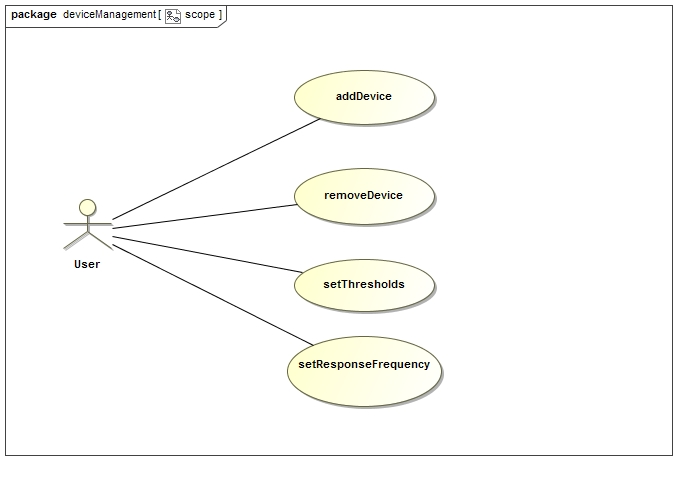
\includegraphics[width=\textwidth]{images/deviceManagementScope.jpg}  \\
			\caption{The scope of functionality required from the Device Management module}
		\end{figure}
		
		A user is able to add and register a new device onto the system, as well as remove old, unnecessary devices. The user can set the measurement thresholds for a specific device, and set how often the device should aim to transfer its data to the web server.
		
	\subsection{User Management}
		\begin{figure}
			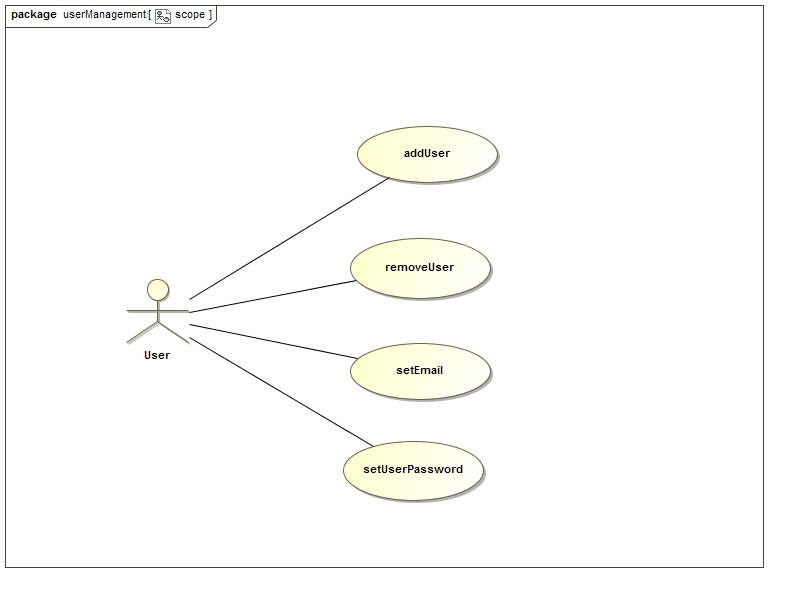
\includegraphics[width=\textwidth]{images/userManagementScope.jpg}  \\
			\caption{The scope of functionality required from the User Management module.}
		\end{figure}
		
		A user is able to add other users to the system, as well as remove old or redundant users. A user can set their personal email address, as well as their password.
		
	\subsection{Data Management}
		\begin{figure}
			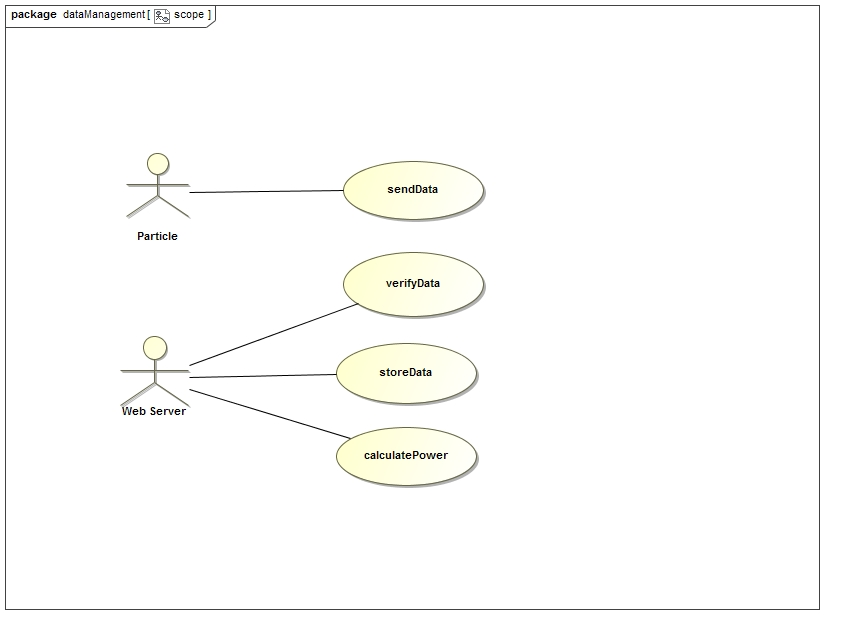
\includegraphics[width=\textwidth]{images/dataManagementScope.jpg}  \\
			\caption{The scope of functionality required from the Data Management module.}
		\end{figure}
		
		The particle device will regularly send the data it has accumulated to the web server. The Web Server can verify the data which it receives, perform the necessary calculations on the received data to calculate desired values, and store the data and results to the persistence service.
		
	\subsection{Reporting Scope}
	\begin{figure}
		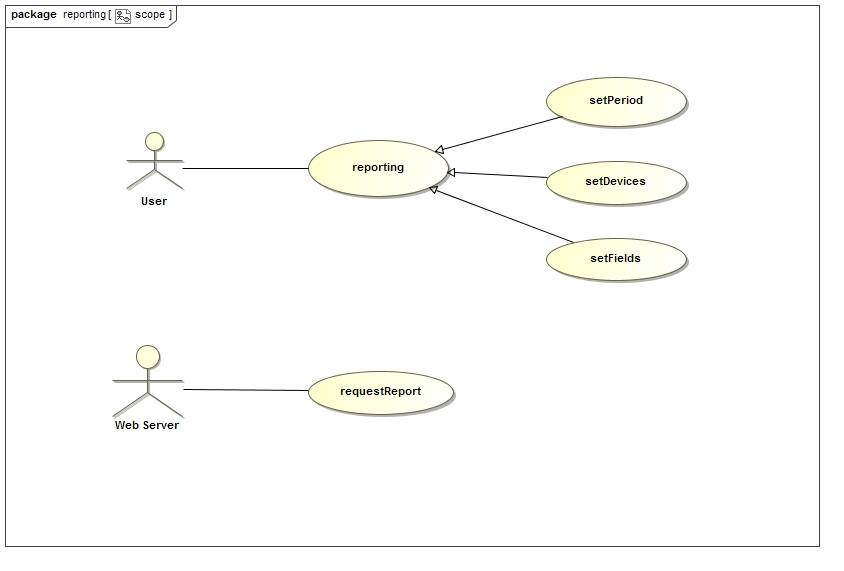
\includegraphics[width=\textwidth]{images/reportingScope.jpg}  \\
		\caption{The scope of functionality required from the reporting module.}
	\end{figure}
	
	The user can request a report made up of data from between a certain period of time, from a certain set of devices, containing a certain set of fields. The web server requests the report from the reporting service, which accesses the required data, compiles and returns the report to the web server.
	\newpage
	\section{Initial Architecture Design}
	\begin{figure}
		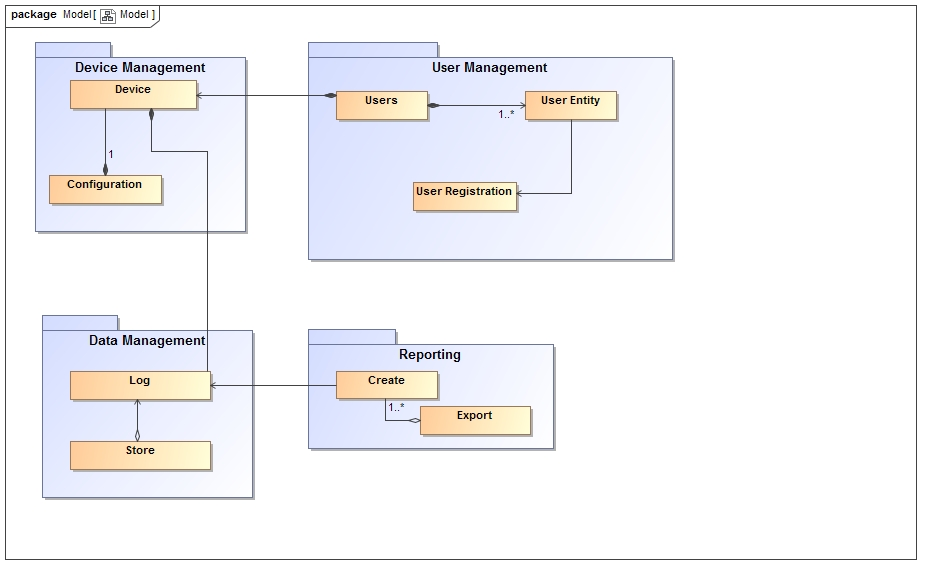
\includegraphics[width=\textwidth]{images/ArchitecturalModel.jpg}  \\
		\caption{The initial Domain Model}
	\end{figure}
	
	\begin{figure}
		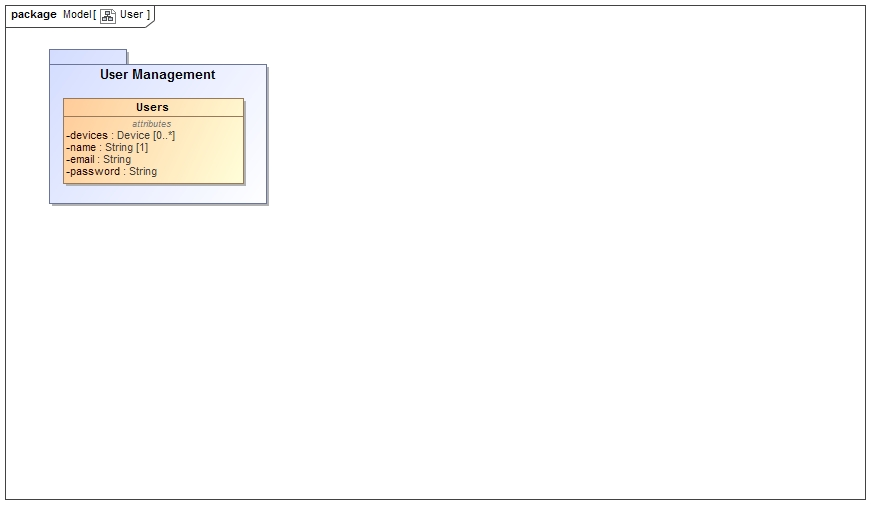
\includegraphics[width=\textwidth]{images/User.jpg}  \\
		\caption{The user package.}
	\end{figure}
	
	\begin{figure}
		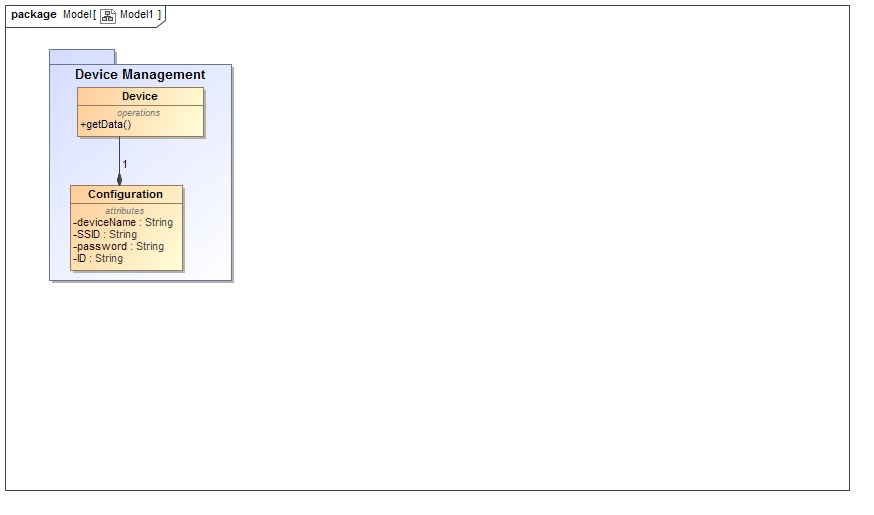
\includegraphics[width=\textwidth]{images/DeviceManagement.jpg}  \\
		\caption{The device management package.}
	\end{figure}
	
	\begin{figure}
		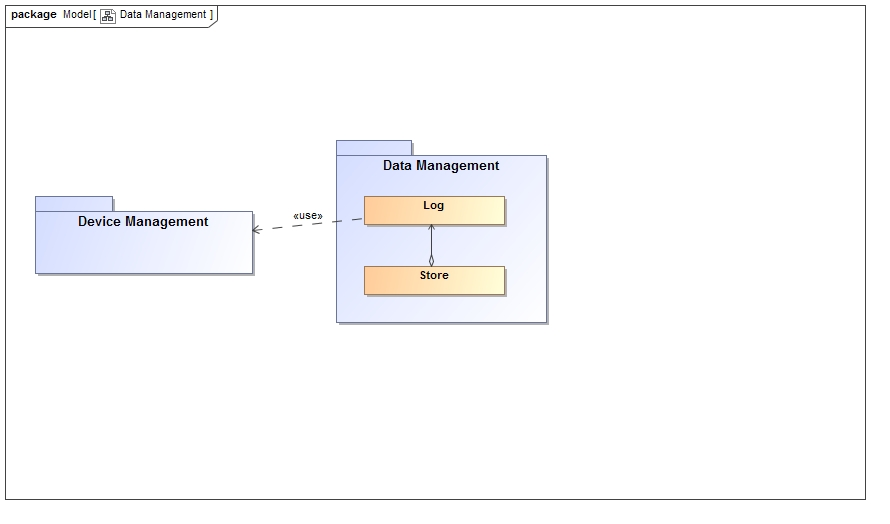
\includegraphics[width=\textwidth]{images/DataManagement.jpg}  \\
		\caption{The data management package.}
	\end{figure}
	
	\begin{figure}
		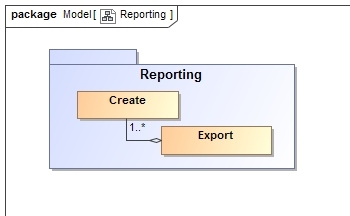
\includegraphics[width=\textwidth]{images/Reporting.jpg}  \\
		\caption{The reporting package.}
	\end{figure}
	\newpage
	\section{Non-functional Requirements}
	\subsection{Quality requirements}
	\textbf{Scalability:}
	Server needs to handle up to 100 000 simultaneous connections from deployed devices.\\
	If any data compression can take place, the server must be able to take advantage of this opportunity.\\
	\\\textbf{Reliability:} The entire system should be portable to ensure close to 100\% up time.\\
	\\\textbf{Quality:}
	Server needs to ensure that data is valid and consistent.\\ The server also needs to identify any inconsistencies in the functionality from the deployed devices and report this immediately.\\
	\\\textbf{Recoverability:}
	If the device goes off-line, data should not be lost.\\
	If the server were to cease function for any reason, a replacement must be put in place within a suitable time period.\\\\
	\textbf{Security:}
	Device communication must be encrypted to avoid interception of sensitive data.
	Unauthorized users must be prevented from accessing the system.\\
	
	
	\newpage
	\section{Proposed Frameworks and Technologies}
	\subsection{Current Transformer data transfers}
	\textit{Serial Peripheral Interface (SPI)} will be used to send data to the photon. SPI is used as a synchronous data bus,
	and uses separate lines for data and a clock which keeps both sides of the SPI in sync. The receiver (particle photon) detects an incoming 
	edge and will immediately data line.\\
	\\There are no alternatives to this technology.
	
	\subsection{Particle Photon}
	The Photon has built in functionalities, coded in C++, which will be used for communications and transfers from the Particle Photon to the server.\\ 
	\\There are no alternatives to this technology.
	
	\subsection{The Web Server}
	One of our choices for a web server is a server compiled with \textit{NodeJS}. NodeJS is run-time environment for server-side web applications. It has an event driven architecture that achieves asynchronous input and output capability.\\
	\\
	It's suitable for this project because it keeps a persistent connection
	from the browser to the server. Any changes made on the data set is immediately propagated through this connection to the client.
	
	\subsection{The Database}
	\textit{Firebase}, is an existing database service. Firebase is a key-value, cloud based database provider. It is tailored to scale on request, the larger the data set gets, the more connections Firebase can handle. A database built on Firebase's infrastructure is accessible through their REST API and bindings for several JavaScript frameworks including AngularJS and Ember.js are available. It provides real-time data synchronization. Firebase servers are located in major city centres around the world this allows for a portable container to be deployed anywhere and ensures that optimal connection speeds will be achieved.\\\\The other option is using \textit{MongoDB}. MongoDB is a document-oriented No-SQL database. Issues with using MongoDB in this system are that it does not provide real-time data synchronization. Therefore extra provisions will have to be made to ensure these capabilities.
	
	\subsection{Data format}
	The data format that will be used is \textit{JSON}. JSON is a lightweight data-interchange format which is also easy to understand and	manipulate. JSON is natively supported across a variety of technologies, it can be used in its raw form with no manipulation required.\\\\Alternatively \textit{MessagePack} could be used. Since MessagePack uses binary serialization to make faster and smaller data compared to JSON.\\
	If data size is a major concern then MessagePack will be a good alternative.
	
	\subsection{Web Application}
	The web application framework will be \textit{Angular.js}. It is a powerful flexible framework with good modularization and extensive module repositories. Angular.JS uses two-way binding and updates the virtual DOM, which could be necessary with the web application. It also works hand in hand with our database technology Firebase.\\
	\\Alternative frameworks would be Ember.js and REACT.
	
	\subsection{Reporting}
	\textit{Google Charts} will be used for reporting. Google Charts provides an API which will allow us to create responsive and intuitive graphical representations of our data with pure Javascript. Coupled with Angular, Google Charts would be a powerful way to ensure that our system functions correctly and that data appears correctly across multiple platforms.
	
\end{document}
